\documentclass[11pt]{article}
\usepackage[utf8]{inputenc}
\usepackage{mathtools}
\usepackage{gensymb}
\usepackage{amsmath}
\usepackage{amssymb}
\usepackage{tikz}
\usepackage{gensymb}
\usetikzlibrary{arrows}

\begin{document}
\section*{Problème}
Étant donné le vecteur $\vec{A}=(2\vec{i}+3\vec{j})\text{ m}$, trouvez le vecteur $\vec{B}$ de module $5\text{ m}$ qui est perpendiculaire à $\vec{A}$ et qui est situé dans les plans suivants : (a) le plan $xz$; (b) le plan $xy$. \cite{problem}

\section*{Résolution}
Ce problème requiert certaines notions de géométrie vectorielle. Si deux vecteurs sont perpendiculaires, le produit scalaire de ces deux vecteurs est nulle. Par définition, le produit scalaire entre deux vecteurs $\vec{A}$ et $\vec{B}$ étant séparé par un angle $\theta$ est :
\begin{equation}
\vec{A}\cdot\vec{B} = ||\vec{A}||\cdot||\vec{B}||\cdot\cos\theta
\end{equation}

Si l'angle $\theta$ est de $90\degree$, on remarque que le produit scalaire est nulle, car $\cos90\degree=0$. Pour le problème, on peut simplifier l'équation (1) :
\begin{equation}
\vec{A}\cdot\vec{B} = 0
\end{equation}

Il existe une deuxième définition du produit scalaire. On peut calculer le produit scalaire entre deux vecteurs $\vec{A}$ et $\vec{B}$ en utilisant les composantes :
\begin{equation}
\vec{A}\cdot\vec{B} = (A_x\cdot B_x)+(A_y\cdot B_y)+(A_z\cdot B_z)
\end{equation}
où $A_x$, $A_y$ et $A_z$ représentent les composantes du vecteur $\vec{A}$, et $B_x$, $B_y$ et $B_z$ représentent les composantes du vecteur $\vec{B}$.\\

Si l'on insère l'équation (2) dans (3), on obtient l'équation :
\begin{equation}
0 = (A_x\cdot B_x)+(A_y\cdot B_y)+(A_z\cdot B_z)
\end{equation}

À partir de l'équation (4), il suffit de substituer les composantes du vecteur $\vec{A}$ dans l'énoncer du problème pour ensuite résoudre les composantes du vecteur $\vec{B}$ :
\begin{equation}
\begin{split}
0 &= (2\cdot B_x)+(3\cdot B_y)+(0\cdot B_z)\\
  &= 2B_x+3B_y+0B_z
\end{split}
\end{equation}
\pagebreak

Il existe une infinité de solutions à cette équation. On peut simplifier $0B_z=0$, mais il est idéale de le garder afin de montrer que $B_z$ peut prendre n'importe quelles valeurs. Afin de trouver une solution précise, il faut prendre compte des restrictions du problème. La partie (a) du problème demande un vecteur $\vec{B}$ dans le plan $xz$, alors il n'y a pas de composante $y$ :

\begin{center}
\documentclass{standalone}
\usepackage{amsmath}
\usepackage{amssymb}
\usepackage{gensymb}
\usepackage{tikz}
\usepackage{esvect}
\usetikzlibrary{arrows}

\begin{document}
\begin{tikzpicture}[x=2.25cm,y=2.2cm,z=1.6cm,>=stealth]
\coordinate (A) at (1.7,1.2,1.0);
\coordinate (B) at (0.7,0.8,-0.7);
% The axes
\draw[->] (xyz cs:x=-2.5) -- (xyz cs:x=2.5) node[above] {$x$};
\draw[->] (xyz cs:y=-2.5) -- (xyz cs:y=2.5) node[right] {$z$};
\draw[->] (xyz cs:z=-2.5) -- (xyz cs:z=2.5) node[above] {$y$};

% The thin ticks
\foreach \coo in {-2.4,-1.9,...,2.4} {
  \draw (\coo,-1.5pt) -- (\coo,1.5pt);
  \draw (-1.0pt,\coo) -- (1.0pt,\coo);
  \draw (xyz cs:y=-0.05pt,z=\coo) -- (xyz cs:y=0.05pt,z=\coo);
}

% The vector
\draw[->] (xyz cs:x=0.0,y=0.0,z=0.0) -- (xyz cs:x=1.7,y= 1.2,z=1.1);
\draw[->] (xyz cs:x=0.0,y=0.0,z=0.0) -- (xyz cs:x=0.7,y=0.8,z=-0.7);

\node[inner sep=1.5pt,label={above:$\vv{OA}$}] at (A) {};
\draw[dashed] (xyz cs:x=0.0,y=0.0,z=1.1) -- node[below] {$2\cos30\degree$} (xyz cs:x=1.7,y=0.0,z=1.1);
\draw[dashed] (xyz cs:x=1.7,y=0.0,z=0.0) -- node[right] {$2\sin30\degree$} (xyz cs:x=1.7,y=0.0,z=1.1);
\draw[dashed] (xyz cs:x=1.7,y=0.0,z=1.1) -- node[right] {$1.2$} (xyz cs:x=1.7,y=1.2,z=1.1);

\node[inner sep=1.5pt,label={above:$\vv{OB}$}] at (B) {};
\draw[dashed] (xyz cs:x=0.0,y=0.0,z=-0.7) -- node[below] {$1\cos315\degree$} (xyz cs:x=0.7,y=0.0,z=-0.7);
\draw[dashed] (xyz cs:x=0.7,y=0.0,z= 0.0) -- node[right] {$1\cos315\degree$} (xyz cs:x=0.7,y=0.0,z=-0.7);
\draw[dashed] (xyz cs:x=0.7,y=0.0,z=-0.7) -- node[above right]  {$0.8$} (xyz cs:x=0.7,y=0.8,z=-0.7);
\end{tikzpicture}
\end{document}
\end{center}

Alors, l'équation (5) se simplifie :
\begin{equation*}
\begin{split}
 0 &= 2B_x+3B_y+0B_z\\
   &= 2B_x+3\cdot 0+0B_z\\
   &= 2B_x+0B_z\\
B_x&= 0B_z = 0
\end{split}
\end{equation*}

Donc, le vecteur $\vec{B}$ n'a pas de composante en $x$ ni en $y$. Cela ne veut pas dire que la composante en $z$ est nulle pour autant. Comme mentionnée plus tôt, la composante $B_z$ peut prendre n'importe quelles valeurs, puisqu'elle est multipliée par le facteur nulle. Une norme de $5\text{ m}$ est demandée pour le vecteur $\vec{B}$, alors on peut simplement associer $B_z=\pm5\text{ m}$. Donc, le vecteur $\vec{B} = 0\vec{i}+0\vec{j}\pm5\vec{k}=\pm5\vec{k}$.\\
\pagebreak

Dans la partie (b) du problème, on cherche un vecteur similaire, mais dans le plan $xy$ , alors il n'y a pas de composante en $z$ :

\begin{center}
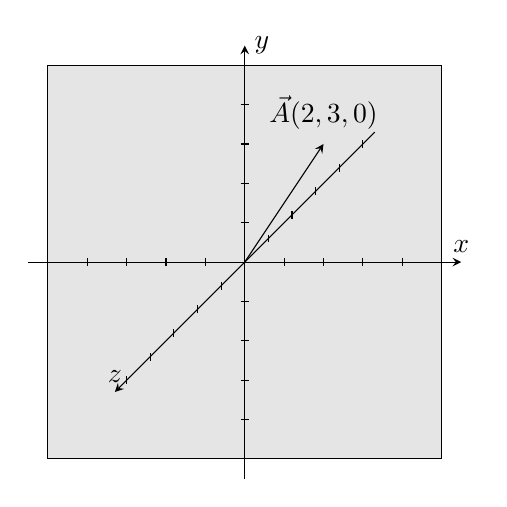
\begin{tikzpicture}[x=0.5cm,y=0.5cm,z=0.3cm,>=stealth]
\coordinate (O) at (0,0,0);
\coordinate (A) at (2,3,0);
\coordinate (P1) at (-5,-5,0);
\coordinate (P2) at (-5, 5,0);
\coordinate (P3) at ( 5, 5,0);
\coordinate (P4) at ( 5,-5,0);
% The axes
\draw[->] (xyz cs:x=-5.5) -- (xyz cs:x= 5.5) node[above] {$x$};
\draw[->] (xyz cs:y=-5.5) -- (xyz cs:y= 5.5) node[right] {$y$};
\draw[->] (xyz cs:z= 5.5) -- (xyz cs:z=-5.5) node[above] {$z$};

% The thin ticks
\foreach \coo in {-5,-4,...,5} {
  \draw (\coo,-1.5pt) -- (\coo,1.5pt);
  \draw (-1.5pt,\coo) -- (1.5pt,\coo);
  \draw (xyz cs:y=-0.10pt,z=\coo) -- (xyz cs:y=0.10pt,z=\coo);
}

% The vector
\draw[->] (O) -- (A);
\node[inner sep=1.5pt,label={above:$\vec{A}(2, 3, 0)$}] at (A) {};

% The plane
\draw[fill=black, fill opacity=0.1] 
	(xyz cs:x=-5,y=-5) -- (xyz cs:x=-5,y= 5) -- 
	(xyz cs:x= 5,y= 5) -- (xyz cs:x= 5,y=-5) -- cycle;
\end{tikzpicture}
\end{center}

Alors, l'équation (4) se simplifie :
\begin{equation}
\begin{split}
 0 &= 2B_x+3B_y+0\cdot 0\\
   &= 2B_x+3B_y
\end{split}
\end{equation}

Contrairement à la partie (a), on obtient une équation avec deux inconnues. Par contre, on demande une norme de $5\text{ m}$. On peut obtenir une deuxième équation afin de résoudre nos deux inconnues :
\begin{alignat*}{3}
                & & ||\vec{B}|| &= \sqrt{B_x^2+B_y^2+B_z^2}\\
\Leftrightarrow & &           5 &= \sqrt{B_x^2+B_y^2}
\end{alignat*}

Donc, la dernière équation et (6) sont nos deux équations à résoudre. On peut isoler $B_x$ dans la dernière.
\begin{alignat*}{3}
                & &     5 &= \sqrt{B_x^2+B_y^2}\\
\Leftrightarrow & &    25 &= B_x^2+B_y^2\\
\Leftrightarrow & & B_x^2 &= 25-B_y^2\\
\Leftrightarrow & &   B_x &= \sqrt{25-B_y^2}
\end{alignat*}
\pagebreak

Ensuite, on substitue $B_x$ dans (6) :
\begin{alignat*}{3}
                & &       0 &= 2B_x+3B_y\\
                & &         &= 2\sqrt{25-B_y^2}+3B_y\\
\Leftrightarrow & &   -3B_y &= 2\sqrt{25-B_y^2}\\
\Leftrightarrow & &  9B_y^2 &= 4(25-B_y^2)\\
                & &         &= 100-4B_y^2\\
\Leftrightarrow & & 13B_y^2 &= 100\\
\Leftrightarrow & &   B_y^2 &= \frac{100}{13}\\
\Leftrightarrow & &     B_y &= \pm\frac{10}{\sqrt{13}}\approx\pm2,77
\end{alignat*}

On peut reprendre (6) et substituer $B_y$ :
\begin{alignat*}{3}
                & &     0 &= 2B_x+3B_y\\
                & &       &= 2B_x+3\left(\pm\frac{10}{\sqrt{13}}\right)\\
\Leftrightarrow & & -2B_x &= \pm\frac{30}{\sqrt{13}}\\
\Leftrightarrow & &   B_x &= \mp\frac{15}{\sqrt{13}}\approx\mp4,16
\end{alignat*}

Finalement, le vecteur $\vec{B}=\mp\dfrac{15}{\sqrt{13}}\vec{i}\pm\dfrac{10}{\sqrt{13}}\vec{i}+0\vec{k}\approx\mp4,16\vec{i}\pm2,77\vec{j}$. Pour conclure, ce problème est très mathématique. La notion de vecteur est très important en physique. Par contre, il est rare que les problèmes de mécanique soit autant centré sur la géométrie vectorielle.
\section*{Bibliographie}
\bibliographystyle{plain}
\renewcommand{\section}[2]{}
\bibliography{bibliography}
\end{document}
